\documentclass[aspectratio=169]{beamer}
\graphicspath{{graphics/}}

\usetheme[progressbar=frametitle]{metropolis}
\usepackage{FiraSans}
\usepackage[style=apa]{biblatex}

\setbeamertemplate{caption}{\raggedright\insertcaption\par}

\renewcommand*{\bibfont}{\footnotesize}
\setbeamertemplate{bibliography item}{}
\addbibresource{bibliography.bib}

\title{Acceleration by Separate-Process Cache\\for Memory-Intensive Algorithms
on FPGA\\via High-Level Synthesis}
\subtitle{Master's Degree Thesis}
\author{Brignone Giovanni \\ \tiny{Supervisor:} \small{Prof.\ Lavagno Luciano}}
\titlegraphic{\hfill\includegraphics[height=2cm]{logopolitonuovo}}
\institute{Politecnico di Torino}
\date{October 21, 2021}

\begin{document}
\begin{frame}
	\maketitle
\end{frame}

%\begin{frame}{Outline}
%	\setbeamertemplate{section in toc}[sections numbered]
%	\tableofcontents[hideallsubsections]
%\end{frame}

{
	\metroset{sectionpage=none}
	\section{Introduction}
}
\begin{frame}{High-Level Synthesis}
	\begin{columns}
		\begin{column}{.45\textwidth}
			\begin{center}
				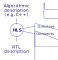
\includegraphics[height=.7\textheight]{hls}
			\end{center}
		\end{column}
		\begin{column}{.45\textwidth}
			\vfill
			\textbf{Primary goals}:
			\begin{itemize}
				\item Productivity
				\item Design space exploration
			\end{itemize}

			\bigskip
			\textbf{Limitations}:
			\begin{itemize}
				\item Low-level control
			\end{itemize}
			\vfill
		\end{column}
	\end{columns}
\end{frame}

\begin{frame}{Memory management}
	\begin{columns}
		\begin{column}{.5\textwidth}
			\textbf{Scratchpad}:
			\begin{itemize}
				\item Manual memory selection
				\item HLS state of the art
			\end{itemize}

			\bigskip

			\textbf{Cache}:
			\begin{itemize}
				\item Automatic full hierarchy exploit
				\item<alert@+> Thesis work objective
			\end{itemize}
		\end{column}
		\begin{column}{.5\textwidth}
			\begin{center}
				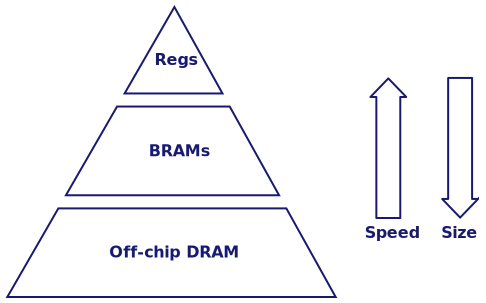
\includegraphics[width=.9\textwidth]{mem_hierarchy}
			\end{center}
		\end{column}
	\end{columns}
\end{frame}

\subsection{Previous work}
\begin{frame}{Previous work}
	\begin{columns}
		\begin{column}{.5\textwidth}
			\vfill
			\textbf{Architecture}:
			\begin{itemize}
				\item Cache inlined in application
			\end{itemize}

			\textbf{Implementation}:
			\begin{itemize}
				\item \texttt{C++} class
			\end{itemize}

			\textbf{User friendliness}:
			\begin{itemize}
				\item \emph{Integrable}: \texttt{operator[]} overload
				\item \emph{Configurable}: template parameters
				\item \emph{Observable}: hit ratio reports
			\end{itemize}
		\end{column}
		\begin{column}{.5\textwidth}
			\begin{center}
				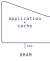
\includegraphics[height=.5\textheight]{liang_arch}
			\end{center}
		\end{column}
	\end{columns}
\end{frame}

\section{Development}
\subsection{Basic architecture}
\begin{frame}{Basic architecture}
	\begin{columns}
		\begin{column}{.55\textwidth}
			\textbf{Objective}:
			\begin{itemize}
				\item Limit application cluttering
			\end{itemize}

			\bigskip
			\textbf{Proposed solution}:
			\begin{itemize}
				\item \underline{Cache:} separate process
					\begin{itemize}
						\item Modeling: threads (SW); dataflow (HW)
						\item Communication: FIFOs
					\end{itemize}
				\item \underline{Application:}
					\begin{enumerate}
						\item Send \emph{request}
						\item Receive \emph{response}
					\end{enumerate}
			\end{itemize}
		\end{column}
		\begin{column}{.5\textwidth}
			\begin{center}
			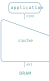
\includegraphics[height=.7\textheight]{complete_arch}
			\end{center}
		\end{column}
	\end{columns}
\end{frame}
\begin{frame}{Basic architecture}
	\begin{columns}
		\begin{column}{.5\textwidth}
			\textbf{Cache process}:
			\begin{itemize}
				\item Optimal pipeline (II=1)
			\end{itemize}
			
			\bigskip
			\textbf{Interface}:
			\begin{itemize}
				\item Scheduler unaware of latency between
					\emph{request} and \emph{response}
				\item Workaround: forced clock cycles
			\end{itemize}
		\end{column}
		\begin{column}{.5\textwidth}
			\begin{center}
				\begin{figure}
					\caption{Original schedule}
					\frame{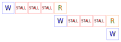
\includegraphics[width=.55\textwidth]{actual_schedule_run}}
				\end{figure}
				\begin{figure}
					\caption{Schedule with workaround}
					\frame{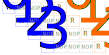
\includegraphics[width=.55\textwidth]{desired_schedule_run}}
				\end{figure}
			\end{center}
		\end{column}
	\end{columns}
\end{frame}
\subsection{Multi-levels architecture}
\begin{frame}{Multi-levels architecture}
	\begin{columns}
		\begin{column}{.5\textwidth}
			\textbf{Objective}:
			\begin{itemize}
				\item Improve read performance
			\end{itemize}
			
			\bigskip
			\textbf{Proposed solution}:
			\begin{itemize}
				\item L1 cache inlined in application
					\begin{itemize}
						\item Write-through
						\item Direct-mapped
					\end{itemize}
			\end{itemize}
		\end{column}
		\begin{column}{.5\textwidth}
			\begin{center}
			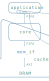
\includegraphics[height=.7\textheight]{l1_arch}
			\end{center}
		\end{column}
	\end{columns}
\end{frame}
\subsection{Multi-ports architecture}
\begin{frame}{Multi-ports architecture}
	\begin{columns}
		\begin{column}{.5\textwidth}
			\textbf{Objective}:
			\begin{itemize}
				\item Efficient application loop unrolling
			\end{itemize}

			\bigskip
			\textbf{Proposed solution}:
			\begin{itemize}
				\item Single L2 cache with multiple ports
				\item Multiple L1 caches
			\end{itemize}
		\end{column}
		\begin{column}{.5\textwidth}
			\begin{center}
			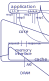
\includegraphics[height=.7\textheight]{multi_ports_arch}
			\end{center}
		\end{column}
	\end{columns}
\end{frame}

\section{Results}
\begin{frame}{Matrix multiplication}
	\begin{columns}
		\begin{column}{.5\textwidth}
			\textbf{Algorithm}:
			\[C = A \times B, \quad A, B, C \in \mathbb{R}^{32 \times 32}\]

			\textbf{Caches configuration}:
			\begin{itemize}
				\item $A$: 1 line of 32 elements
				\item $B$: 32 lines of 32 elements\\(direct mapped)
				\item $C$: 1 line of 32 elements
			\end{itemize}
		\end{column}
		\begin{column}{.5\textwidth}
			\begin{center}
				\includegraphics[width=\textwidth]{plot}
			\end{center}
		\end{column}
	\end{columns}
\end{frame}

\section{Summary}
\begin{frame}{Summary}
	\textbf{Achieved results}:
	\begin{itemize}
		\item Multi-process modeling for HLS
		\item Design space extended by cache
	\end{itemize}

	\bigskip
	\textbf{Future work}:
	\begin{itemize}
		\item Fix interface schedule: RTL implementation
	\end{itemize}
\end{frame}

\begin{frame}{References}
	\nocite{*}
	\printbibliography[heading=none]
\end{frame}

\end{document}

